\documentclass[border=10pt]{standalone}
%%%<
\usepackage{verbatim}
%%%>
\usepackage{pgfplots}
\pgfplotsset{width=7cm,compat=1.8}
\usepgfplotslibrary{polar}
\begin{comment}
:Title: A polar plot
:Tags: 2D;Polar plots;Manual
:Author: Christian Feuersänger
:Slug: polar-axes

The polar library allows to draw polar axes and plot types
relying on polar coordinates, represented by angle (in
degrees or, optionally, in radians) and radius.

The code is from the PGFPlots 1.10 manual: "5.9.1 Polar Axes".
\end{comment}
\begin{document}
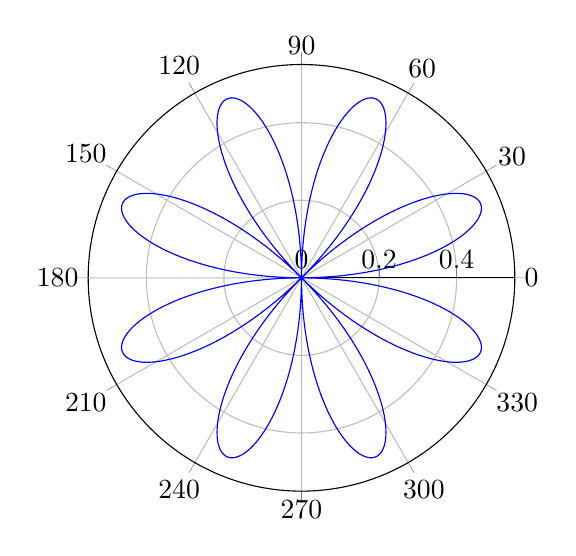
\begin{tikzpicture}
	\begin{polaraxis}
	\addplot+[mark=none,domain=0:720,samples=600] 
		{sin(2*x)*cos(2*x)}; 
	% equivalent to (x,{sin(..)cos(..)}), i.e.
	% the expression is the RADIUS
	\end{polaraxis}
\end{tikzpicture}
\end{document}
